\documentclass[lualatex,hyperref={pdfencoding=auto}]{beamer}
\usepackage[czech]{babel}

\usetheme[fei]{vsb}

\title[Komprese stromových struktur]{Komprese stromových struktur}
\subtitle{Semestrální projekt}
\author{Marek Beran}
\institute[VŠB-TUO]{VŠB -- Technická univerzita Ostrava\\\vspace{2mm}marek.beran.st@vsb.cz}
\date[23.~5.~2019]{23.~května 2019}

\showboxdepth=5

\begin{document}

\begin{frame}
	\tableofcontents
	% Komentář: Stručně projdu osnovu prezentace - od úvodu přes teoretický základ, 
	% návrh architektury a implementaci až po výsledky experimentů a závěry.
\end{frame}

\section{Úvod a motivace}
\begin{frame}{Motivace projektu}
  \begin{columns}
    \begin{column}{0.6\textwidth}
      \begin{itemize}
        \item Komprese dat - klíčová oblast informatiky
        \item Řešení pro sekvenční data běžné (text, multimédia)
        \item Stromové struktury představují specifickou výzvu
        \item<2-> Přirozený jazyk obsahuje opakující se syntaktické vzorce
        \item<2-> Syntaktické stromy - možný cíl optimalizované komprese?
      \end{itemize}
    \end{column}
    \begin{column}{0.4\textwidth}
      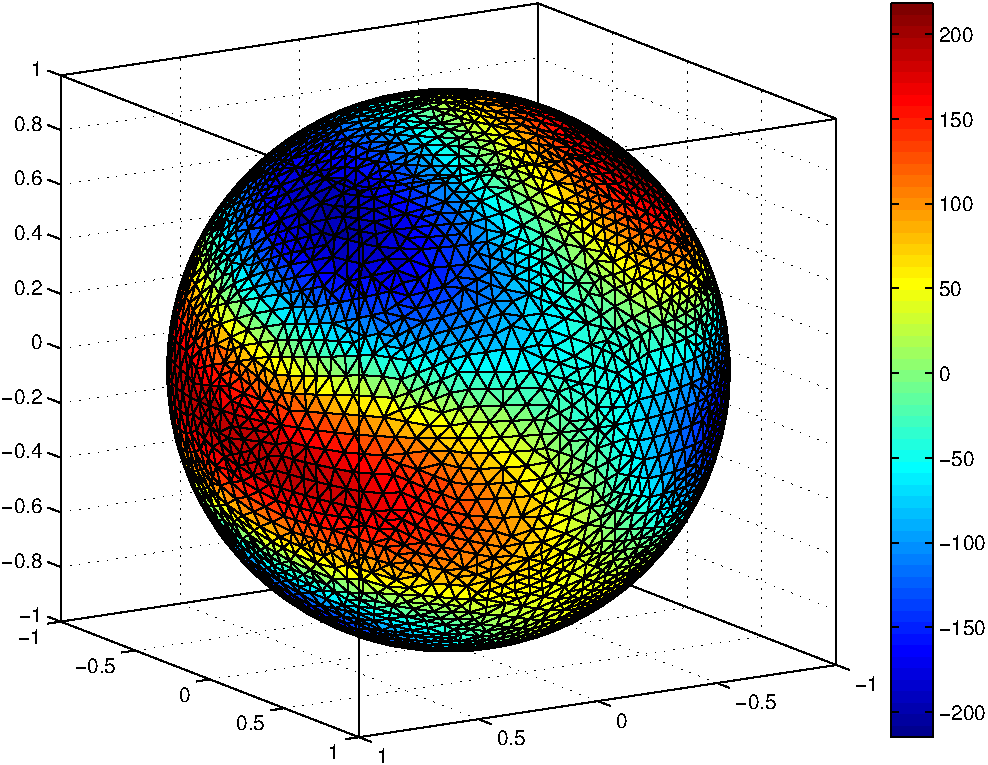
\includegraphics[width=\textwidth]{fig/sphere_mix_real.pdf}
      % Zde by byl obrázek zachycující závislostní strom věty
    \end{column}
  \end{columns}
  % Komentář: Vysvětlím, proč je komprese stromových struktur zajímavým tématem,
  % zejména v kontextu zpracování přirozeného jazyka. Ukážu příklad závislostního
  % stromu a naznačím, jak se v jazyce opakují určité struktury.
\end{frame}

\begin{frame}{Cíle projektu}
  \begin{itemize}
    \item Navrhnout a implementovat knihovnu pro kompresi stromových struktur
    \item Zaměřit se na syntaktické stromy vytvořené z přirozeného jazyka
    \item Ověřit hypotézu o možné efektivní kompresi využitím opakujících se vzorců
    \item Srovnat různé přístupy ke kompresi stromových struktur
    \item<2-> Naivní hypotéza: Velikost komprimovaných stromů roste logaritmicky s délkou textu
  \end{itemize}
  \vspace{5mm}
  \begin{center}
    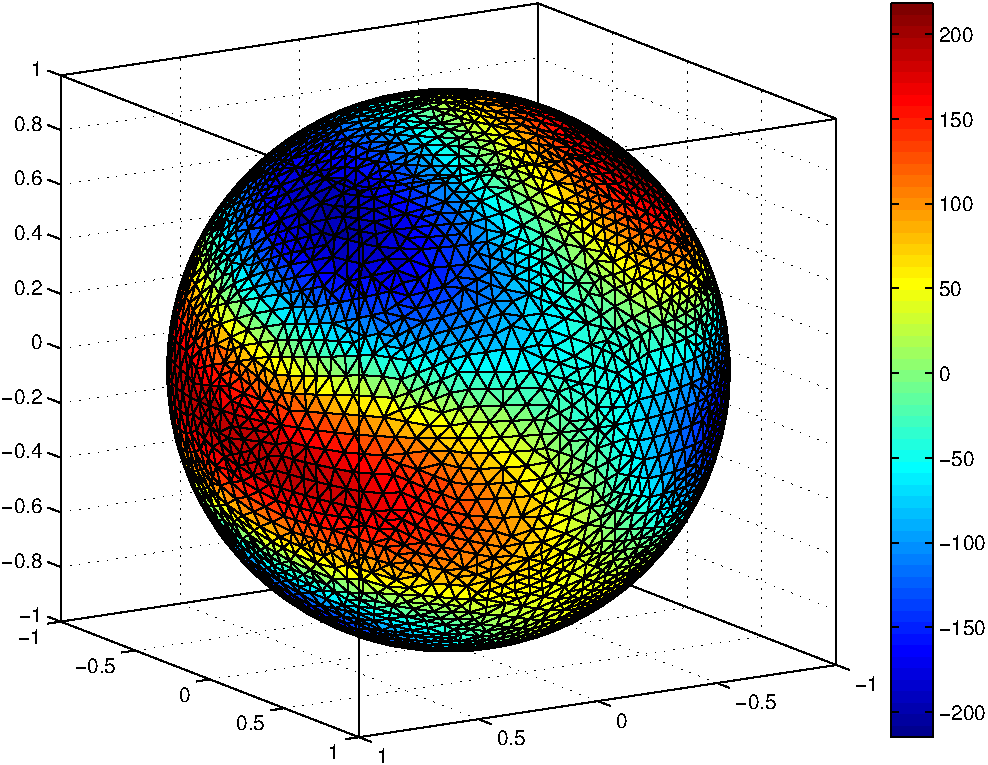
\includegraphics[width=0.7\textwidth]{fig/sphere_mix_real.pdf}
    % Zde by byl ilustrační graf zobrazující logaritmickou křivku růstu 
    % velikosti komprimovaných dat vzhledem k velikosti vstupu
  \end{center}
  % Komentář: Představím hlavní cíle projektu a vysvětlím naivní hypotézu
  % o logaritmickém růstu velikosti komprimovaných dat s rostoucí délkou vstupu.
  % Zdůrazním, že ověření této hypotézy je jedním z cílů práce.
\end{frame}

\section{Nástroje a metody}
\begin{frame}{Použité technologie a nástroje}
  \begin{columns}
    \begin{column}{0.5\textwidth}
      \textbf{Implementační prostředí:}
      \begin{itemize}
        \item Programovací jazyk C\#
        \item Objektově orientovaný přístup
        \item Vzor Pipes and Filters
      \end{itemize}
      \vspace{3mm}
      \textbf{NLP nástroje:}
      \begin{itemize}
        \item MorphoDiTa - morfologická analýza
        \item UDPipe - dependency parsing
      \end{itemize}
    \end{column}
    \begin{column}{0.5\textwidth}
      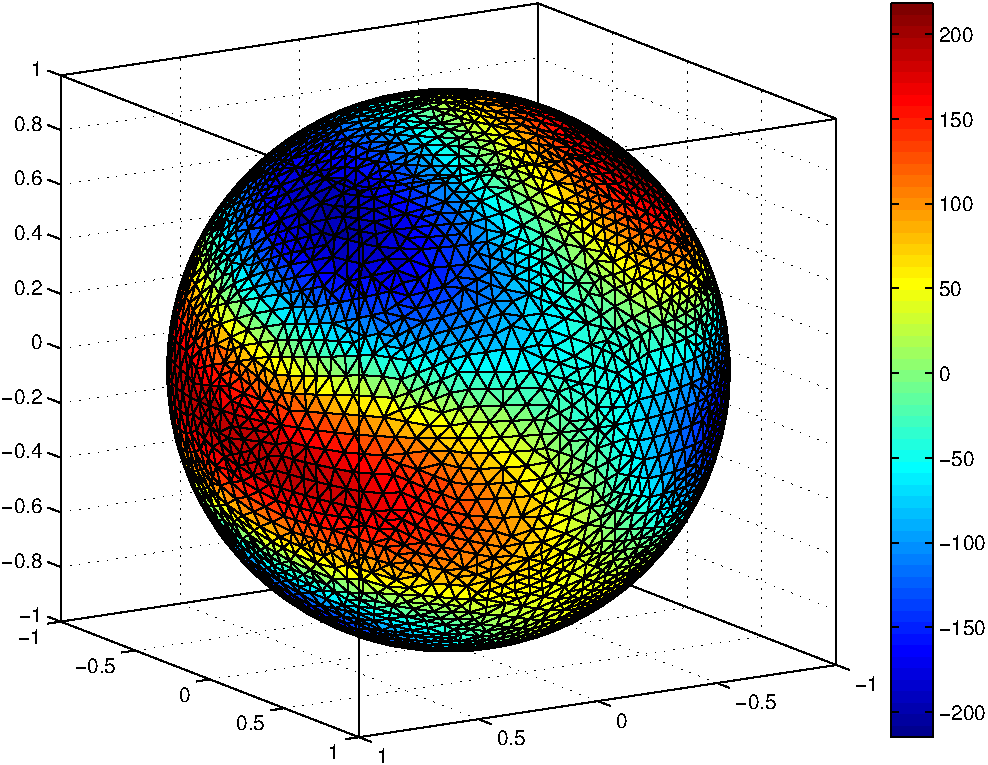
\includegraphics[width=\textwidth]{fig/sphere_mix_real.pdf}
      % Zde by bylo schéma znázorňující UDPipe pipeline
    \end{column}
  \end{columns}
  % Komentář: Popíšu technologický stack projektu - proč jsem zvolil C#,
  % jaké knihovny jsem využil pro zpracování přirozeného jazyka a proč.
  % Vysvětlím, jak UDPipe vytváří závislostní stromy, které jsou základem
  % pro následnou kompresi.
\end{frame}

\begin{frame}{Syntaktická analýza}
  \begin{columns}
    \begin{column}{0.55\textwidth}
      \textbf{Dependency parsing:}
      \begin{itemize}
        \item Metoda pro vytvoření syntaktického stromu
        \item Uzly = slova, hrany = vztahy mezi slovy
        \item Zachycuje gramatickou strukturu věty
        \item Klíčový pro vytvoření vstupních dat
      \end{itemize}
      \vspace{3mm}
      \textbf{Z věty na strom:}
      \begin{enumerate}
        \item Tokenizace a lemmatizace
        \item POS tagging
        \item Dependency parsing
      \end{enumerate}
    \end{column}
    \begin{column}{0.45\textwidth}
      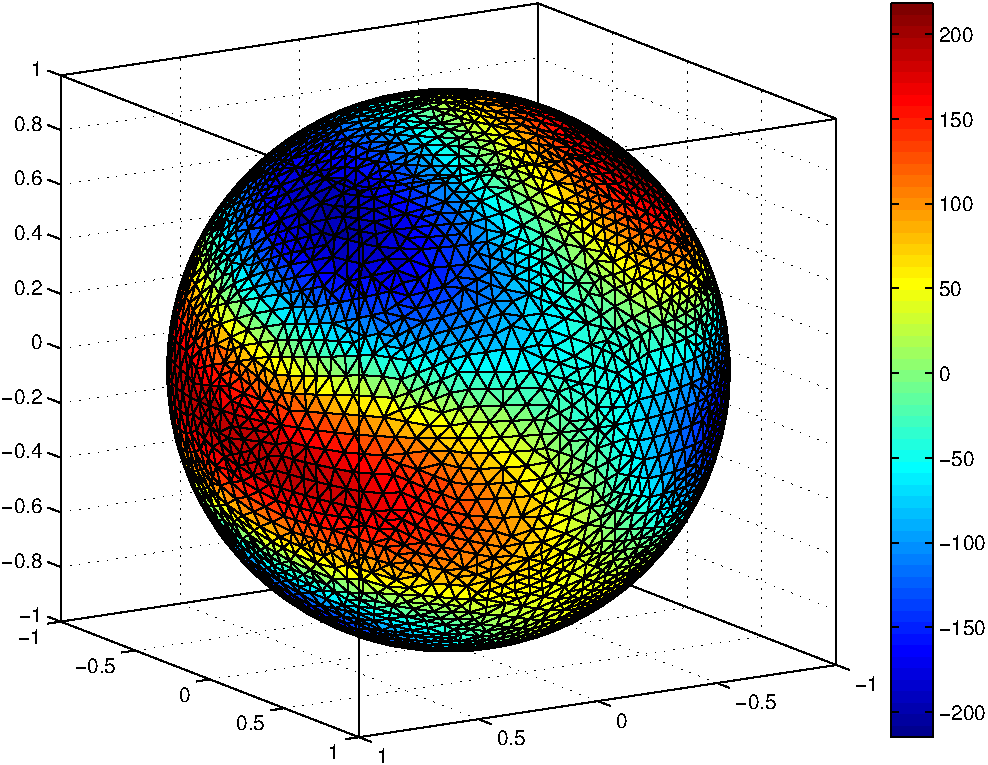
\includegraphics[width=\textwidth]{fig/sphere_mix_real.pdf}
      % Zde by byl obrázek procesu parsování konkrétní věty
    \end{column}
  \end{columns}
  % Komentář: Vysvětlím princip dependency parsingu a jak tvoří základ pro
  % stromové struktury, které komprimuji. Ukážu na příkladu, jak se z běžné věty
  % vytvoří závislostní strom a jaké informace v sobě nese.
\end{frame}

\section{Architektura a implementace}
\begin{frame}{Návrh knihovny}
  \begin{center}
    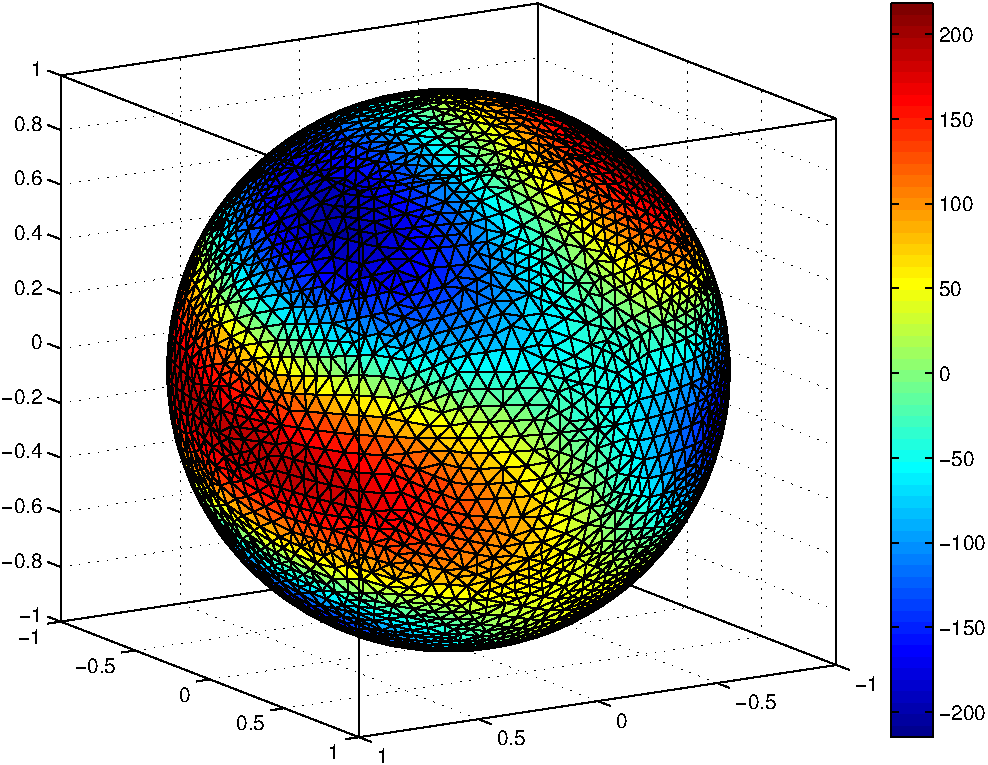
\includegraphics[width=0.9\textwidth]{fig/sphere_mix_real.pdf}
    % Zde by byl zjednodušený diagram architektury knihovny
  \end{center}
  \vspace{3mm}
  \textbf{Klíčové principy:}
  \begin{itemize}
    \item Modularita - jednotlivé komponenty lze kombinovat
    \item Rozšiřitelnost - snadné přidání nových algoritmů
    \item Znovupoužitelnost - podpora různých typů stromů
  \end{itemize}
  % Komentář: Představím architekturu knihovny a zdůrazním její modularitu.
  % Vysvětlím, že architektura umožňuje snadné přidávání nových algoritmů
  % a testování různých přístupů, což je klíčové pro výzkumný charakter práce.
\end{frame}

\begin{frame}{Pipeline zpracování}
  \begin{center}
    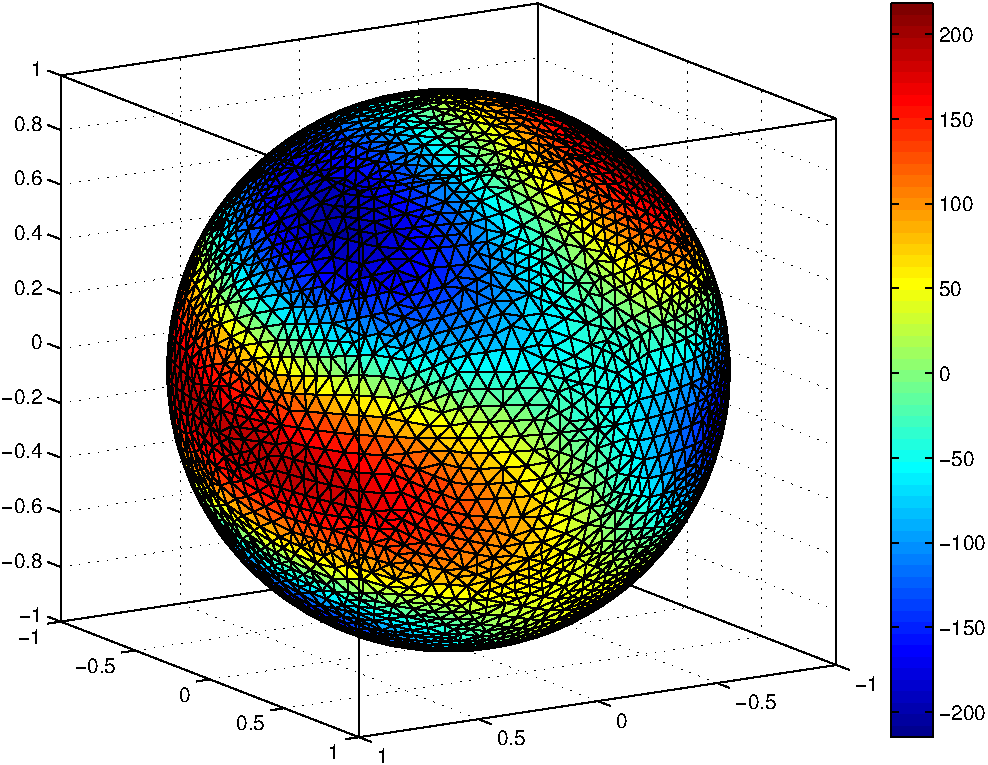
\includegraphics[width=\textwidth]{fig/sphere_mix_real.pdf}
    % Zde by bylo schéma znázorňující pipeline zpracování dat
  \end{center}
  \vspace{3mm}
  \textbf{Hlavní scénáře:}
  \begin{itemize}
    \item \textbf{Kompresní větev:} Text → Analýza → Stromová struktura → Komprese → Uložení
    \item \textbf{Dekompresní větev:} Načtení → Dekomprese → Ověření → Uložení
  \end{itemize}
  % Komentář: Podrobněji vysvětlím procesy komprese a dekomprese, jak jsou
  % implementovány v knihovně. Ukážu příklad, jak data procházejí jednotlivými
  % filtry v pipeline a jak se transformují.
\end{frame}

\section{Kompresní algoritmy}
\begin{frame}{Implementované algoritmy}
  \begin{columns}
    \begin{column}{0.5\textwidth}
      \textbf{Algoritmus RePair:}
      \begin{itemize}
        \item Recursive Pair - nahrazování opakujících se párů
        \item Vytváření gramatických pravidel
      \end{itemize}
      \vspace{2mm}
      \textbf{Dva hlavní přístupy:}
      \begin{enumerate}
        \item Přímá komprese stromu bez linearizace
        \item Linearizace + aplikace RePair
      \end{enumerate}
    \end{column}
    \begin{column}{0.5\textwidth}
      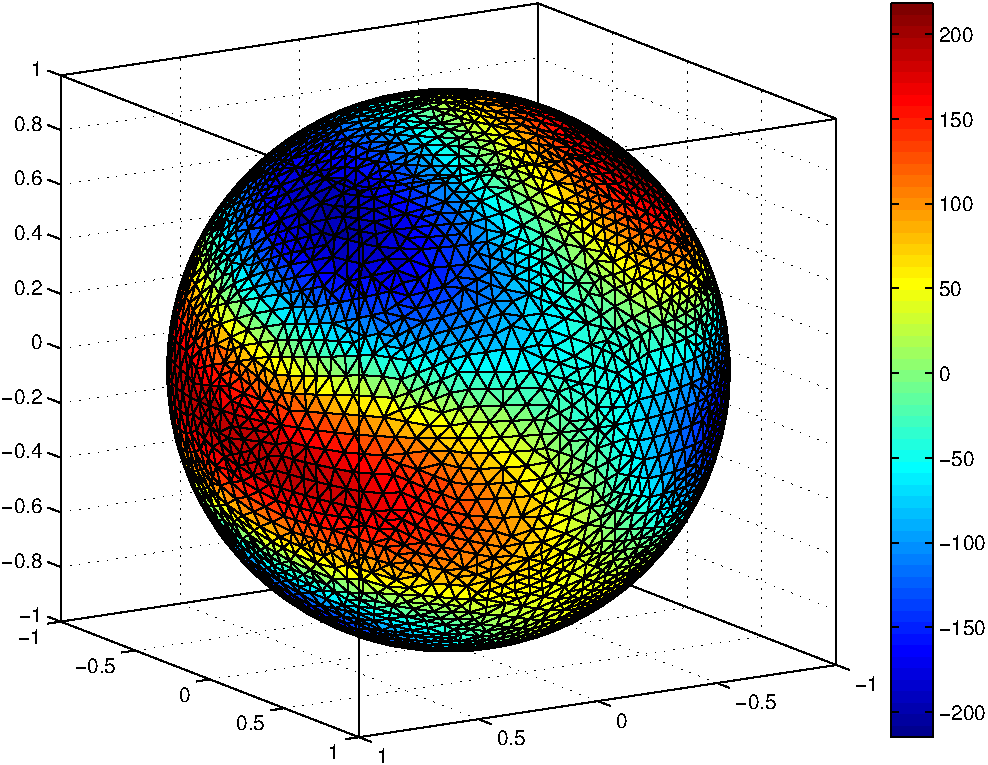
\includegraphics[width=\textwidth]{fig/sphere_mix_real.pdf}
      % Zde by byla ilustrace algoritmu RePair
    \end{column}
  \end{columns}
  % Komentář: Představím algoritmus RePair jako základ pro implementované
  % kompresní metody. Vysvětlím dva hlavní přístupy - přímou kompresi stromové
  % struktury a přístup s linearizací. Nastíním výhody a nevýhody obou přístupů.
\end{frame}

\begin{frame}{TreeRePair - komprese bez linearizace}
  \begin{columns}
    \begin{column}{0.55\textwidth}
      \textbf{Základní varianta:}
      \begin{enumerate}
        \item Identifikace opakujících se podstromů
        \item Výběr nejčastějších
        \item Nahrazení neterminály
        \item Vytvoření gramatických pravidel
      \end{enumerate}
      \vspace{2mm}
      \textbf{Optimalizovaná varianta:}
      \begin{itemize}
        \item Komplexní metrika pro výběr podstromů
        \item Prioritizace podle velikosti, četnosti a hloubky
        \item Paměťové optimalizace
      \end{itemize}
    \end{column}
    \begin{column}{0.45\textwidth}
      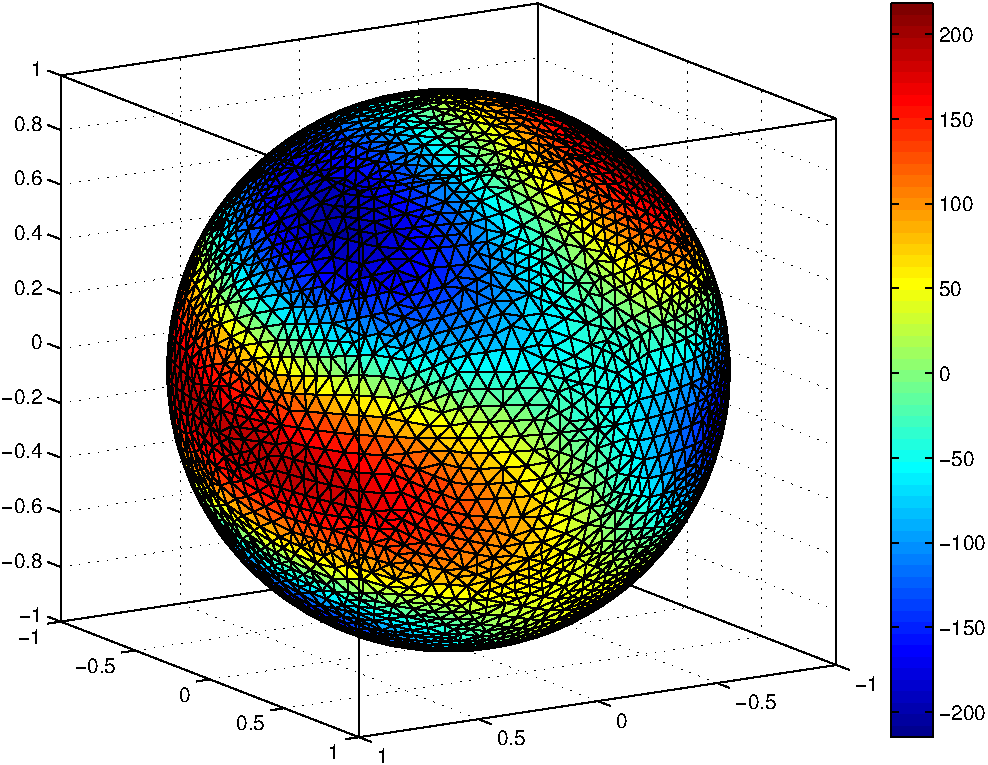
\includegraphics[width=\textwidth]{fig/sphere_mix_real.pdf}
      % Zde by byl příklad komprese podstromu
    \end{column}
  \end{columns}
  % Komentář: Podrobněji vysvětlím přístup TreeRePair, který pracuje přímo
  % se stromovou strukturou. Ukážu na příkladu, jak algoritmus identifikuje
  % a nahrazuje opakující se podstromy. Zdůrazním optimalizace, které jsem
  % implementoval pro zlepšení výkonu.
\end{frame}

\begin{frame}{Linearizace a RePair}
  \begin{columns}
    \begin{column}{0.55\textwidth}
      \textbf{Základní varianta:}
      \begin{enumerate}
        \item Preorder průchod stromem
        \item Vytvoření lineární sekvence
        \item Aplikace RePair na sekvenci
      \end{enumerate}
      \vspace{2mm}
      \textbf{Optimalizovaná varianta:}
      \begin{itemize}
        \item Vylepšený způsob linearizace
        \item Rozšíření na n-gramy místo digramů
        \item Kontextově citlivé nahrazování
        \item Optimalizace gramatiky
      \end{itemize}
    \end{column}
    \begin{column}{0.45\textwidth}
      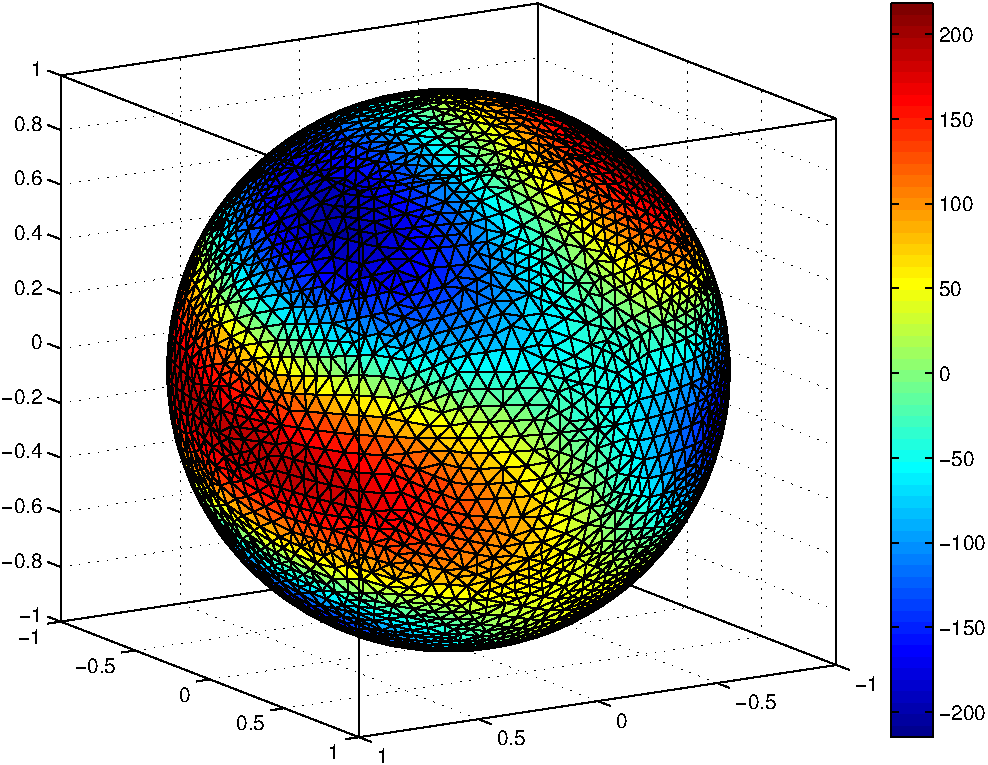
\includegraphics[width=\textwidth]{fig/sphere_mix_real.pdf}
      % Zde by byla ilustrace procesu linearizace stromu
    \end{column}
  \end{columns}
  % Komentář: Popíšu alternativní přístup s linearizací stromu následovanou
  % aplikací algoritmu RePair. Vysvětlím, jak probíhá linearizace a jaké
  % optimalizace jsem implementoval. Porovnám oba přístupy z hlediska
  % teoretických výhod a nevýhod.
\end{frame}

\section{Výsledky experimentů}
\begin{frame}{Metodika testování}
  \textbf{Testovací data:}
  \begin{itemize}
    \item Technická dokumentace - specifický jazyk, časté opakování výrazů
    \item Próza - proměnlivý styl, složitější větné konstrukce
    \item Právní dokumenty - formální jazyk, přísná pravidla struktury
  \end{itemize}
  \vspace{2mm}
  \textbf{Měřené metriky:}
  \begin{itemize}
    \item Kompresní poměr - poměr velikosti komprimovaných dat ku původním
    \item Kompresní zisk - procentuální úspora místa
    \item Doba komprese a dekomprese
    \item Paměťová náročnost
  \end{itemize}
  % Komentář: Představím metodiku testování - jaké typy dat jsem použil
  % a proč jsou vhodné pro ověření hypotéz. Vysvětlím měřené metriky
  % a jejich význam pro hodnocení efektivity komprese.
\end{frame}

\begin{frame}{Porovnání kompresních poměrů}
  \begin{center}
    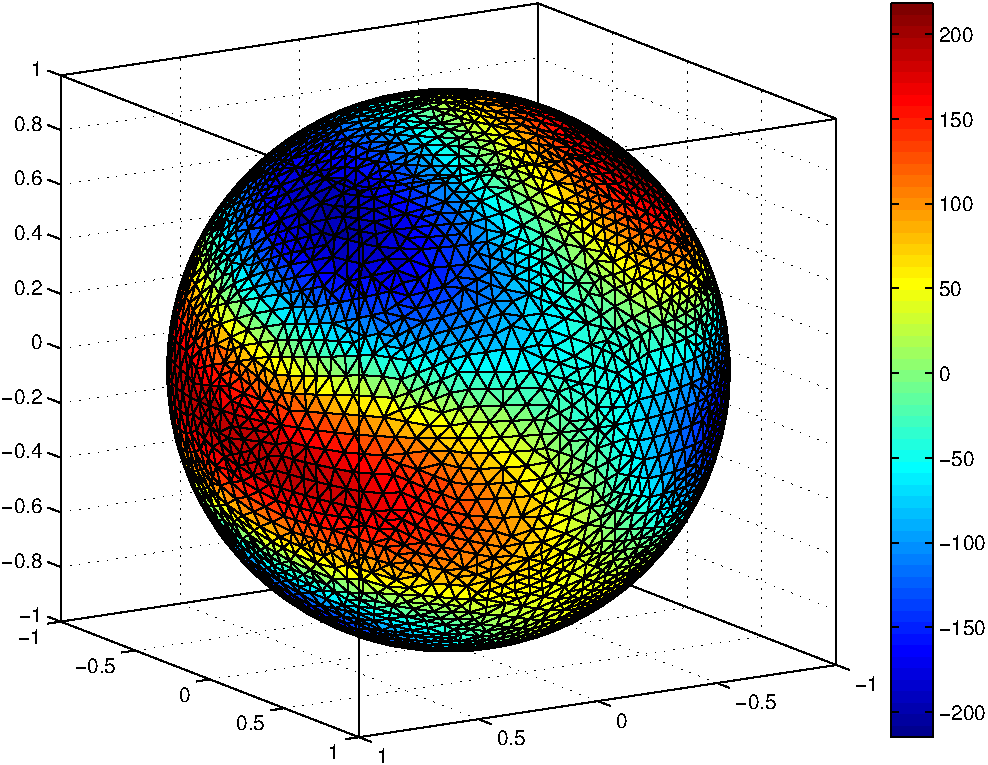
\includegraphics[width=0.9\textwidth]{fig/sphere_mix_real.pdf}
    % Zde by byl graf porovnávající kompresní poměry různých algoritmů
  \end{center}
  \vspace{3mm}
  \begin{columns}
    \begin{column}{0.5\textwidth}
      \textbf{Nejlepší výsledky:}
      \begin{itemize}
        \item Opt. linearizace + RePair: 1,19 (průměr)
        \item Opt. komprese bez lin.: 1,34 (průměr)
        \item Próza: Nejlepší výsledky (1,05 - 1,19)
      \end{itemize}
    \end{column}
    \begin{column}{0.5\textwidth}
      \textbf{Úspěšná komprese:}
      \begin{itemize}
        \item 9,05% případů s opt. linearizací
        \item 5,26% případů s opt. kompresí bez lin.
        \item Hodnoty < 1,0 znamenají skutečnou kompresi
      \end{itemize}
    \end{column}
  \end{columns}
  % Komentář: Představím hlavní výsledky experimentů z hlediska kompresních
  % poměrů. Ukážu, který algoritmus dosáhl nejlepších výsledků a pro jaké
  % typy dat. Zdůrazním, že skutečná komprese (hodnota < 1,0) byla dosažena
  % jen v malém procentu případů.
\end{frame}

\begin{frame}{Vliv velikosti vstupních dat}
  \begin{center}
    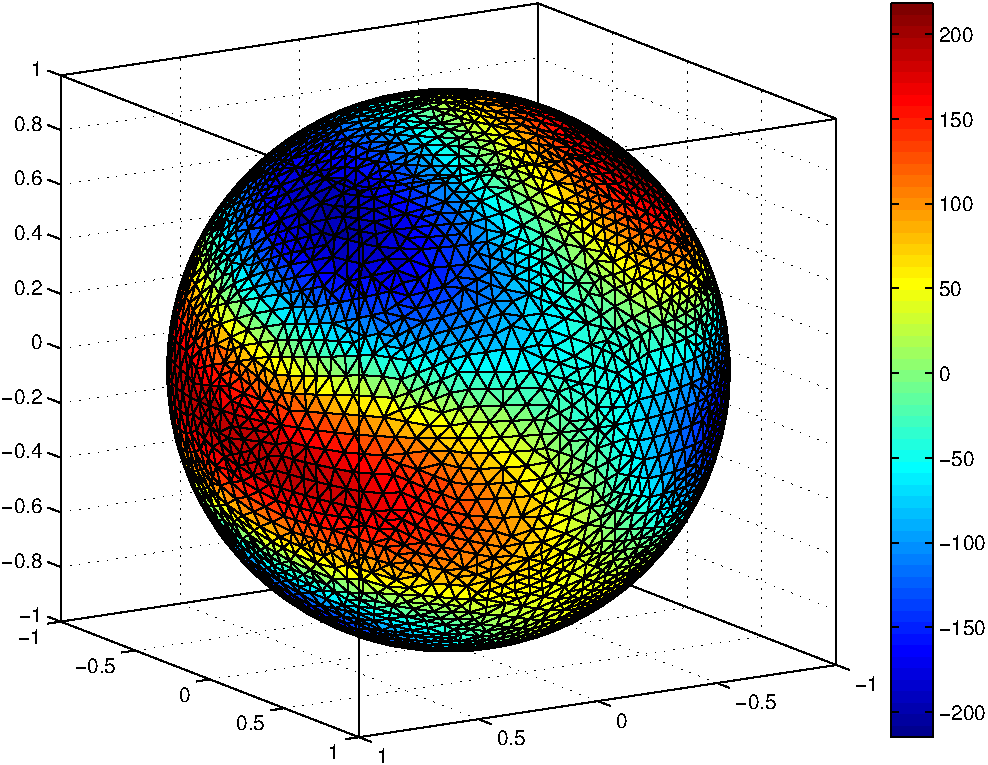
\includegraphics[width=0.9\textwidth]{fig/sphere_mix_real.pdf}
    % Zde by byl graf zobrazující závislost kompresního poměru na velikosti vstupu
  \end{center}
  \vspace{3mm}
  \textbf{Klíčová zjištění:}
  \begin{itemize}
    \item Větší soubory - lepší kompresní poměry
    \item Velmi velké soubory (>100KB) - nejlepší výsledky
    \item Malé soubory (<1KB) - komprese neefektivní
    \item Naznačuje logaritmický trend, ale ne tak výrazný jak předpokládáno
  \end{itemize}
  % Komentář: Vysvětlím, jak velikost vstupních dat ovlivňuje efektivitu
  % komprese. Ukážu, že větší soubory obecně vedou k lepším kompresním poměrům,
  % což částečně potvrzuje původní hypotézu, ale ne v takové míře, jak bylo
  % očekáváno.
\end{frame}

\begin{frame}{Vliv optimalizací a linearizace}
  \begin{columns}
    \begin{column}{0.5\textwidth}
      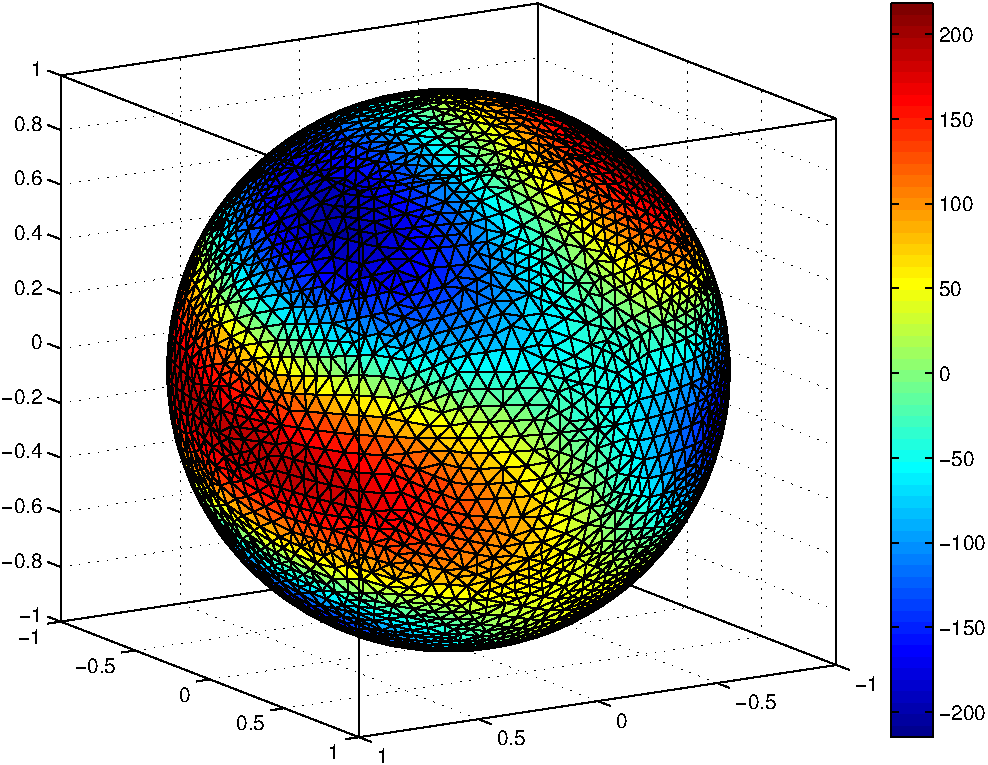
\includegraphics[width=\textwidth]{fig/sphere_mix_real.pdf}
      % Graf vlivu optimalizací
    \end{column}
    \begin{column}{0.5\textwidth}
      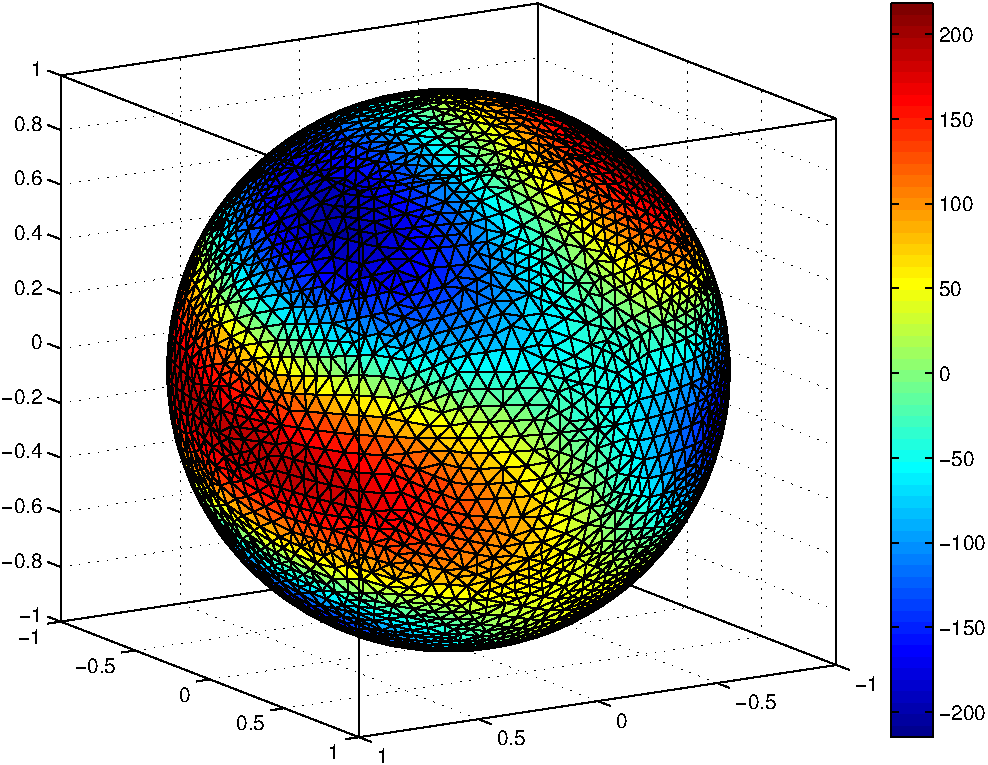
\includegraphics[width=\textwidth]{fig/sphere_mix_real.pdf}
      % Graf vlivu linearizace
    \end{column}
  \end{columns}
  \vspace{3mm}
  \textbf{Vliv optimalizací:}
  \begin{itemize}
    \item Zlepšení průměrného kompresního poměru o 14-24\%
    \item Největší přínos u právních dokumentů
  \end{itemize}
  \textbf{Vliv linearizace:}
  \begin{itemize}
    \item Algoritmy s linearizací obecně efektivnější
    \item Výraznější rozdíl u větších souborů
  \end{itemize}
  % Komentář: Podrobněji analyzuji vliv implementovaných optimalizací
  % a význam linearizace pro efektivitu komprese. Ukážu, jak výrazně
  % tyto faktory ovlivnily výsledné kompresní poměry a pro jaké typy
  % dat měly největší přínos.
\end{frame}

\begin{frame}{Časová náročnost}
  \begin{center}
    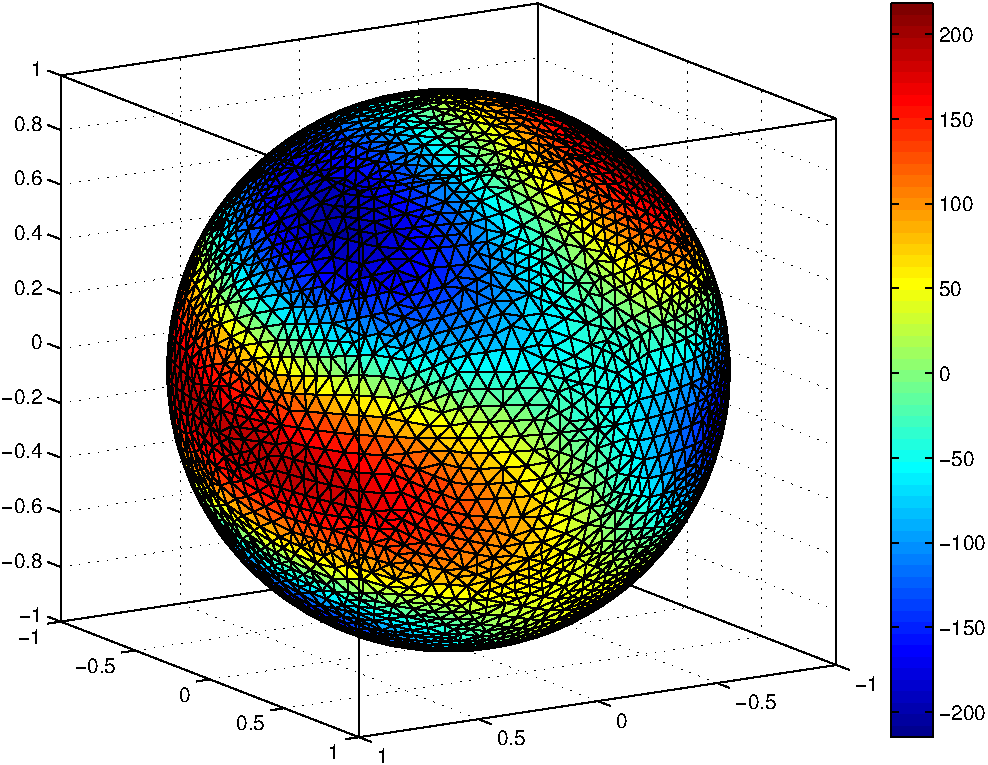
\includegraphics[width=0.85\textwidth]{fig/sphere_mix_real.pdf}
    % Zde by byl graf zobrazující časovou náročnost různých algoritmů
  \end{center}
  \vspace{2mm}
  \textbf{Pozorování:}
  \begin{itemize}
    \item Varianta bez linearizace - nejpomalejší (zejména pro velké soubory)
    \item Linearizace s RePair - výrazně rychlejší
    \item Přímá kompromis rychlost vs. kvalita komprese
    \item Optimalizované varianty - vyšší časová náročnost, lepší výsledky
  \end{itemize}
  % Komentář: Analyzuji časovou náročnost jednotlivých algoritmů a ukážu
  % trade-off mezi rychlostí a kvalitou komprese. Vysvětlím, proč jsou
  % algoritmy bez linearizace výrazně pomalejší a jak optimalizace
  % ovlivňují dobu zpracování.
\end{frame}

\section{Závěr}
\begin{frame}{Shrnutí výsledků}
  \textbf{Hlavní zjištění:}
  \begin{itemize}
    \item Komprese stromových struktur představuje značnou výzvu
    \item Nejlepších výsledků dosahuje optimalizovaná linearizace s RePair
    \item Skutečná komprese (poměr < 1,0) dosažena jen v ~9\% případů
    \item Větší soubory umožňují efektivnější kompresi
    \item Optimalizace přinesly výrazné zlepšení oproti základním variantám
  \end{itemize}
  \vspace{3mm}
  \textbf{Ověření hypotézy:}
  \begin{itemize}
    \item Logaritmický trend potvrzen, ale ne tak výrazný
    \item Opakující se vzorce existují, ale jejich využití není tak efektivní
  \end{itemize}
  % Komentář: Shrnu hlavní výsledky projektu a zhodnotím, nakolik byla
  % potvrzena původní hypotéza. Vysvětlím, proč komprese stromových struktur
  % nepřinesla tak dobré výsledky, jak bylo očekáváno, a jaké faktory
  % to ovlivnily.
\end{frame}

\begin{frame}{Možnosti dalšího vývoje}
  \begin{columns}
    \begin{column}{0.6\textwidth}
      \textbf{Směry budoucího výzkumu:}
      \begin{itemize}
        \item Adaptivní přepínání mezi variantami algoritmů
        \item Další optimalizace linearizace
        \item Paralelizace zpracování
        \item Hybridní přístupy kombinující různé metody
        \item Specializace na konkrétní typy textů
        \item Ztrátová komprese stromových struktur
      \end{itemize}
    \end{column}
    \begin{column}{0.4\textwidth}
      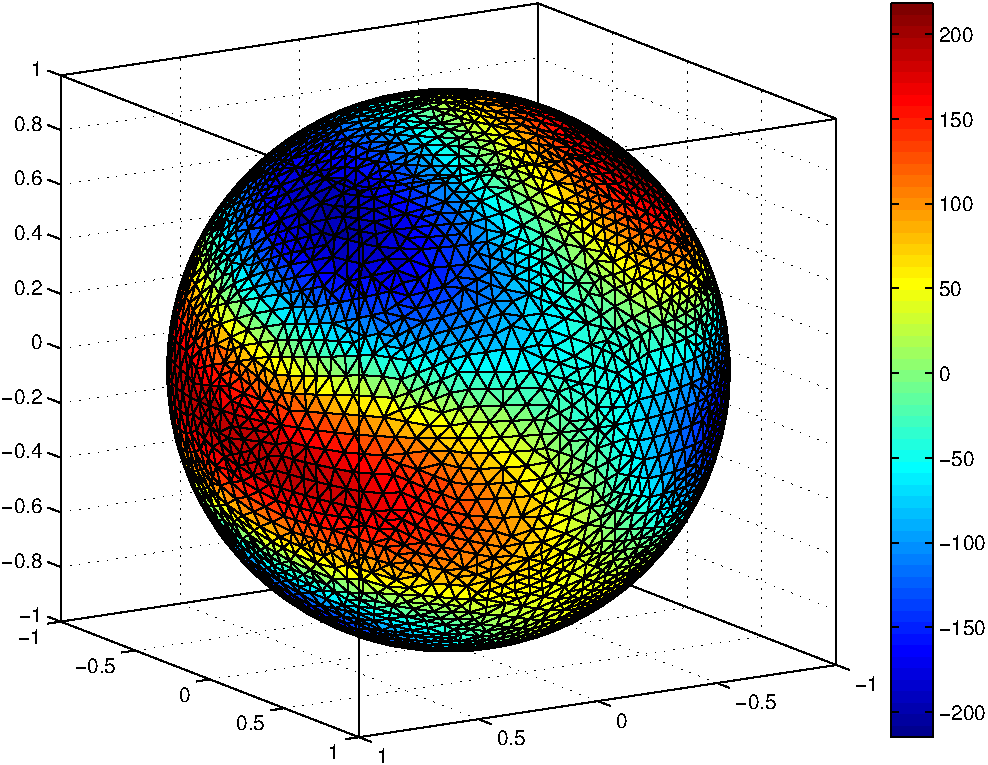
\includegraphics[width=\textwidth]{fig/sphere_mix_real.pdf}
      % Ilustrace budoucích směrů výzkumu
    \end{column}
  \end{columns}
  % Komentář: Nastíním možné směry dalšího výzkumu a vývoje na základě
  % získaných poznatků. Vysvětlím, jaké přístupy by mohly vést k lepším
  % výsledkům a jak by mohla být knihovna dále rozšířena nebo optimalizována.
\end{frame}
\end{document}
